\documentclass[a4paper, 11pt]{article}
\usepackage{comment} 
\usepackage{fullpage}
\usepackage{amsmath} 
\usepackage{amssymb} 
\usepackage{mathtools}
\usepackage{siunitx}
\usepackage{xfrac}
\usepackage{icomma}
\usepackage[section,below]{placeins}
\usepackage[labelfont=bf,font=small,width=0.9\textwidth]{caption}
\usepackage{subcaption}
\usepackage{graphicx}
\usepackage{grffile}
\usepackage{float}
\floatplacement{figure}{htbp}
\floatplacement{table}{htbp}
\usepackage{booktabs}
\usepackage{hyperref}
\sisetup{separate-uncertainty=true}

\begin{document}
\noindent
\centerline{\small{\textsc{Michigan State University}}} \\
\large{\textbf{CMSE/CSE 822 – Parallel Computing \hfill Fall 2019 \\
Homework 6}} \\
Alexander Harnisch \\
\noindent\makebox[\linewidth]{\rule{\textwidth}{0.4pt}}

{\noindent\Large{\textbf{Parallel Bucket Sort with MPI}}}
\section*{Part 1}
General comment: In the instructions it says ``These are the default names in
the git repository. It is essential that you do not change the directory
structure or file names.''. However, that is not the case. I provided the files
as asked for, and additionally a file called
\textit{bucket\_sort\_v2\_squared.c} which is the version used in Part 2. If
you don't pull that one and run my makefile without specifying the target, it
will fail. My all directive also tries to build the squared version.

\subsection*{1.}
See code in repository.

\subsection*{2.}
Figure~\ref{fig:p1_v1_speedup} and Figure~\ref{fig:p1_v2_speedup} shows the
speedup and efficieny for \textit{bucket\_sort\_v1.c} and
\textit{bucket\_sort\_v2.c} respectively. The base case is the one using one
full socket with 14 cores. The total and partial execution times can be seen in
Figure~\ref{fig:p1_v1_times} and Figure~\ref{fig:p1_v2_times} all parts of the
code, that are executed on multiple cores are reported as averages in these
plots. The plots have many interesting features, but since you don't ask for a
description I won't type it out. The only question the assignment asks is:

\textbf{Which phases in your code are
the root causes of the performance difference that you observe between your
bucket sort implementations?}

The root causes are the generation, binning and distribution phases. Everything
else is unchanged after all. \textit{bucket\_sort\_v2.c} is much faster for
large $n$ because the binning and generation are also parallelized. However, as
always, that creates additional overhead (in this case especially in
distribution time) that is too expensive for small problem sizes. We can
clearly see that by comparing the execution time for the smallest problem size
between the two versions. 

\begin{figure}
  \centering
  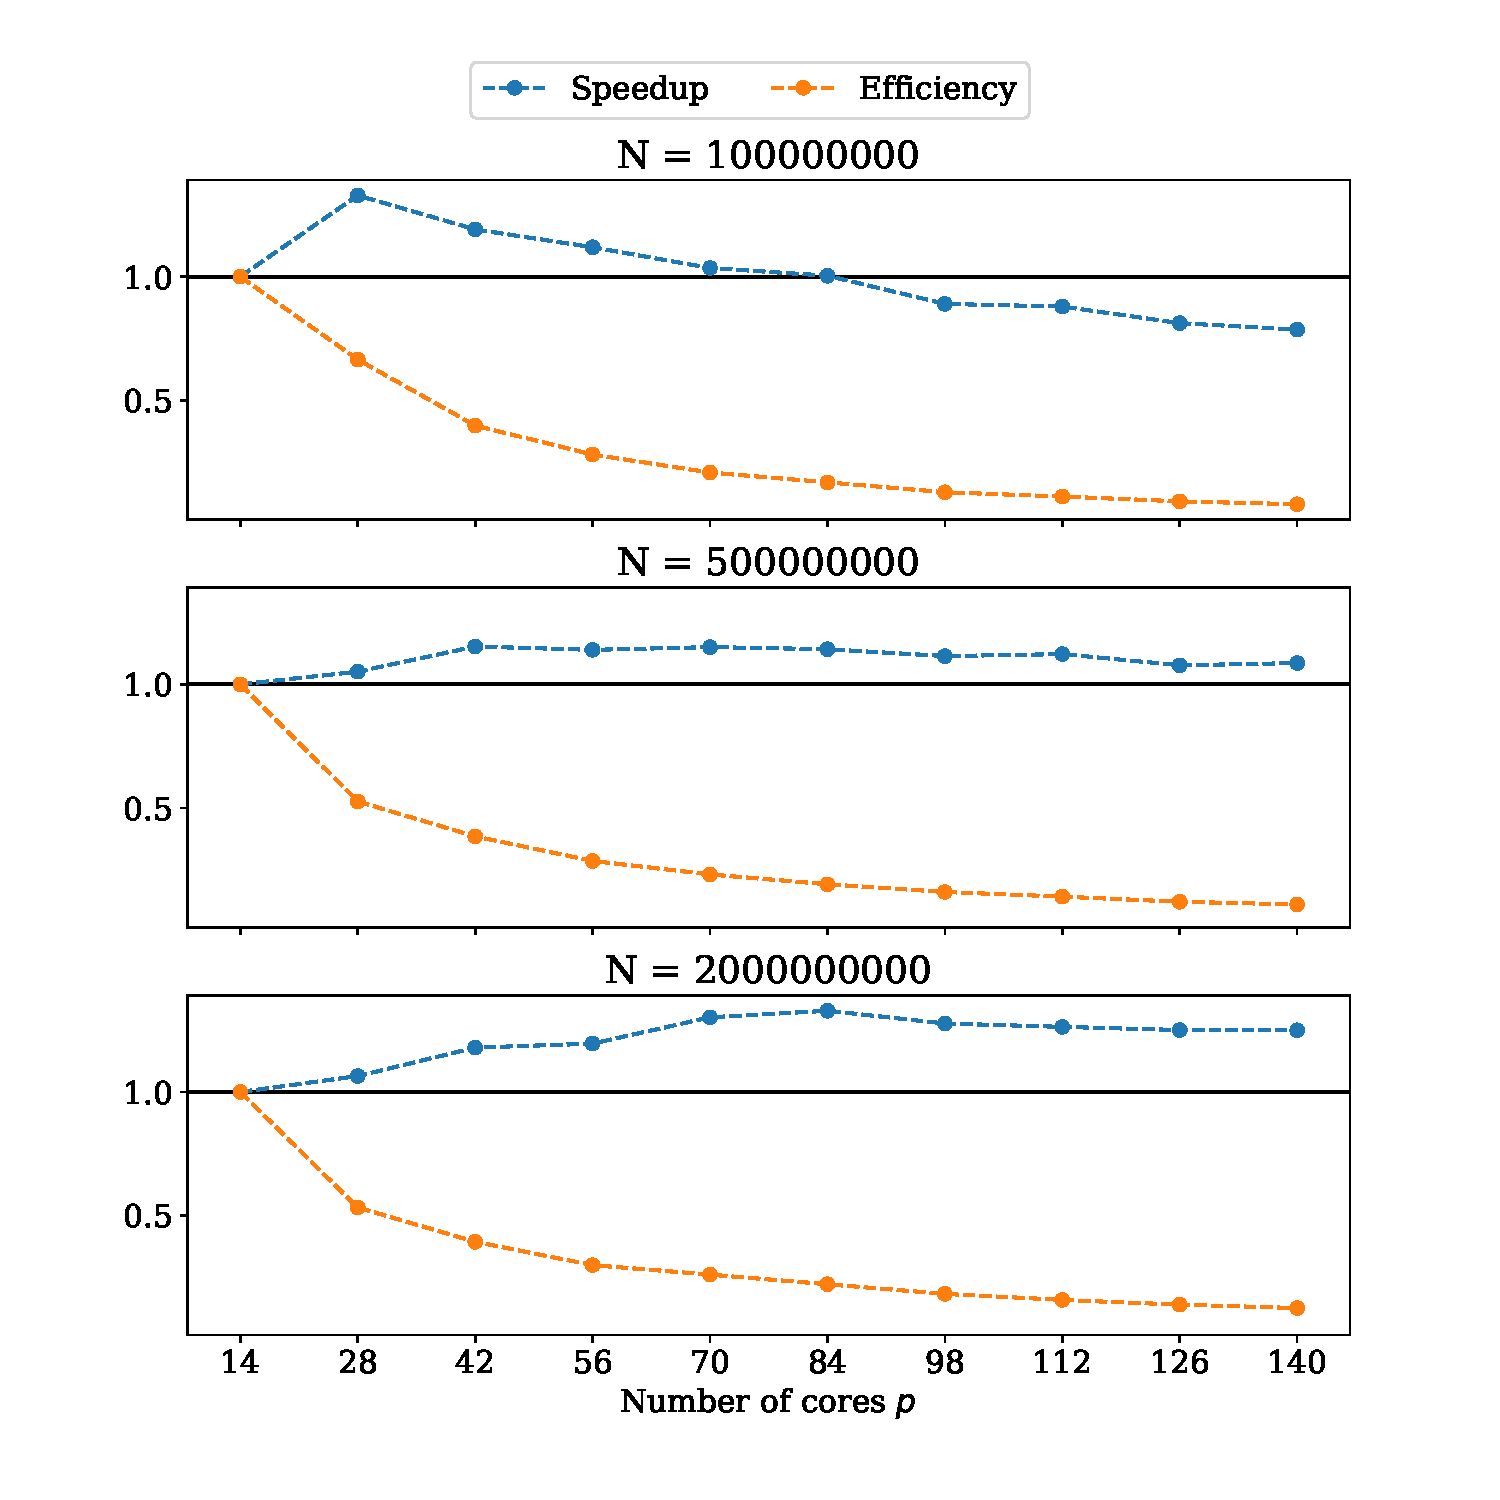
\includegraphics[width=\textwidth]{../part_1/plot/v1_speedup.pdf}
  \caption{Speedup and efficiency of \textit{bucket\_sort\_v1.c} for different
    number of cores $p$.}
  \label{fig:p1_v1_speedup}
\end{figure}
\begin{figure}
  \centering
  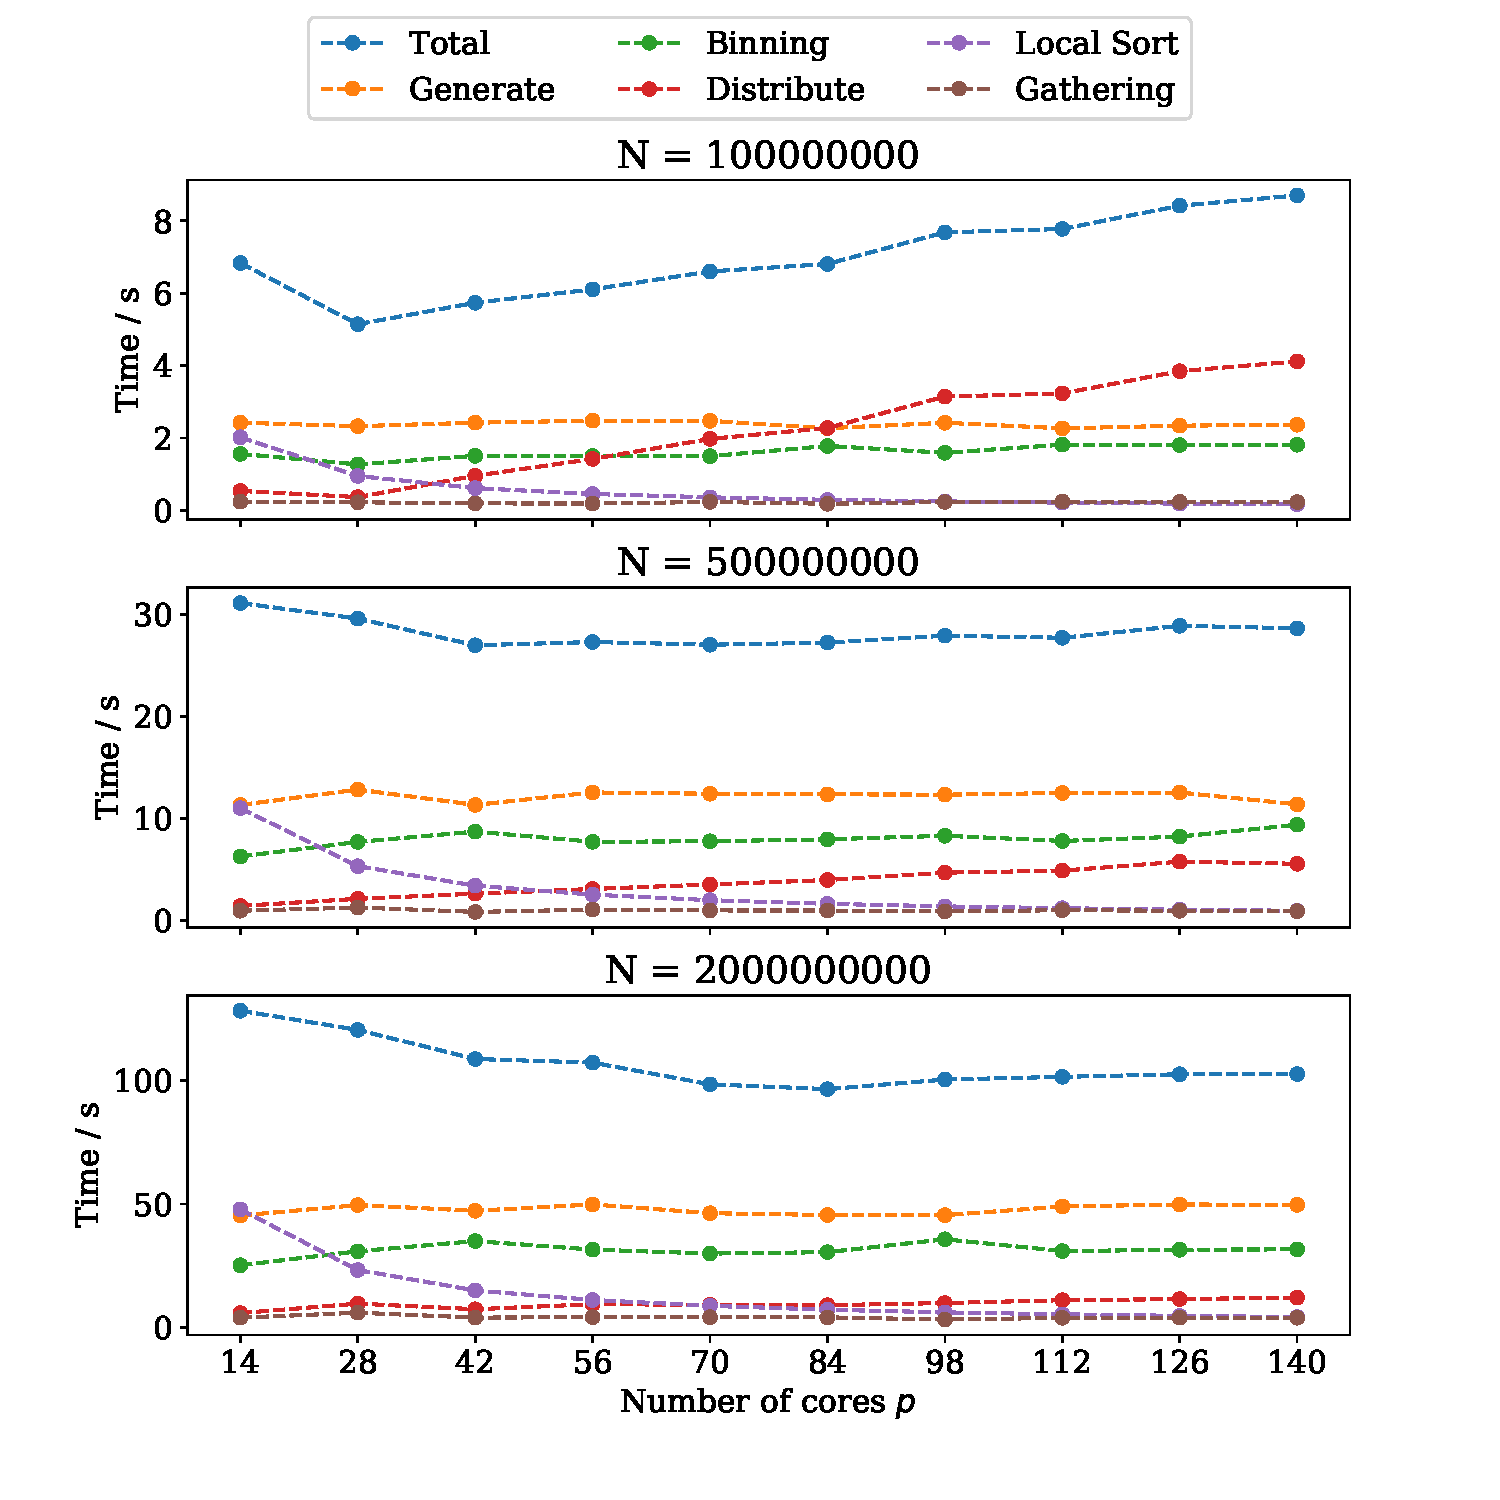
\includegraphics[width=\textwidth]{../part_1/plot/v1_times.pdf}
  \caption{Execution times of \textit{bucket\_sort\_v1.c} for different number
  of cores $p$.}
  \label{fig:p1_v1_times}
\end{figure}

\begin{figure}
  \centering
  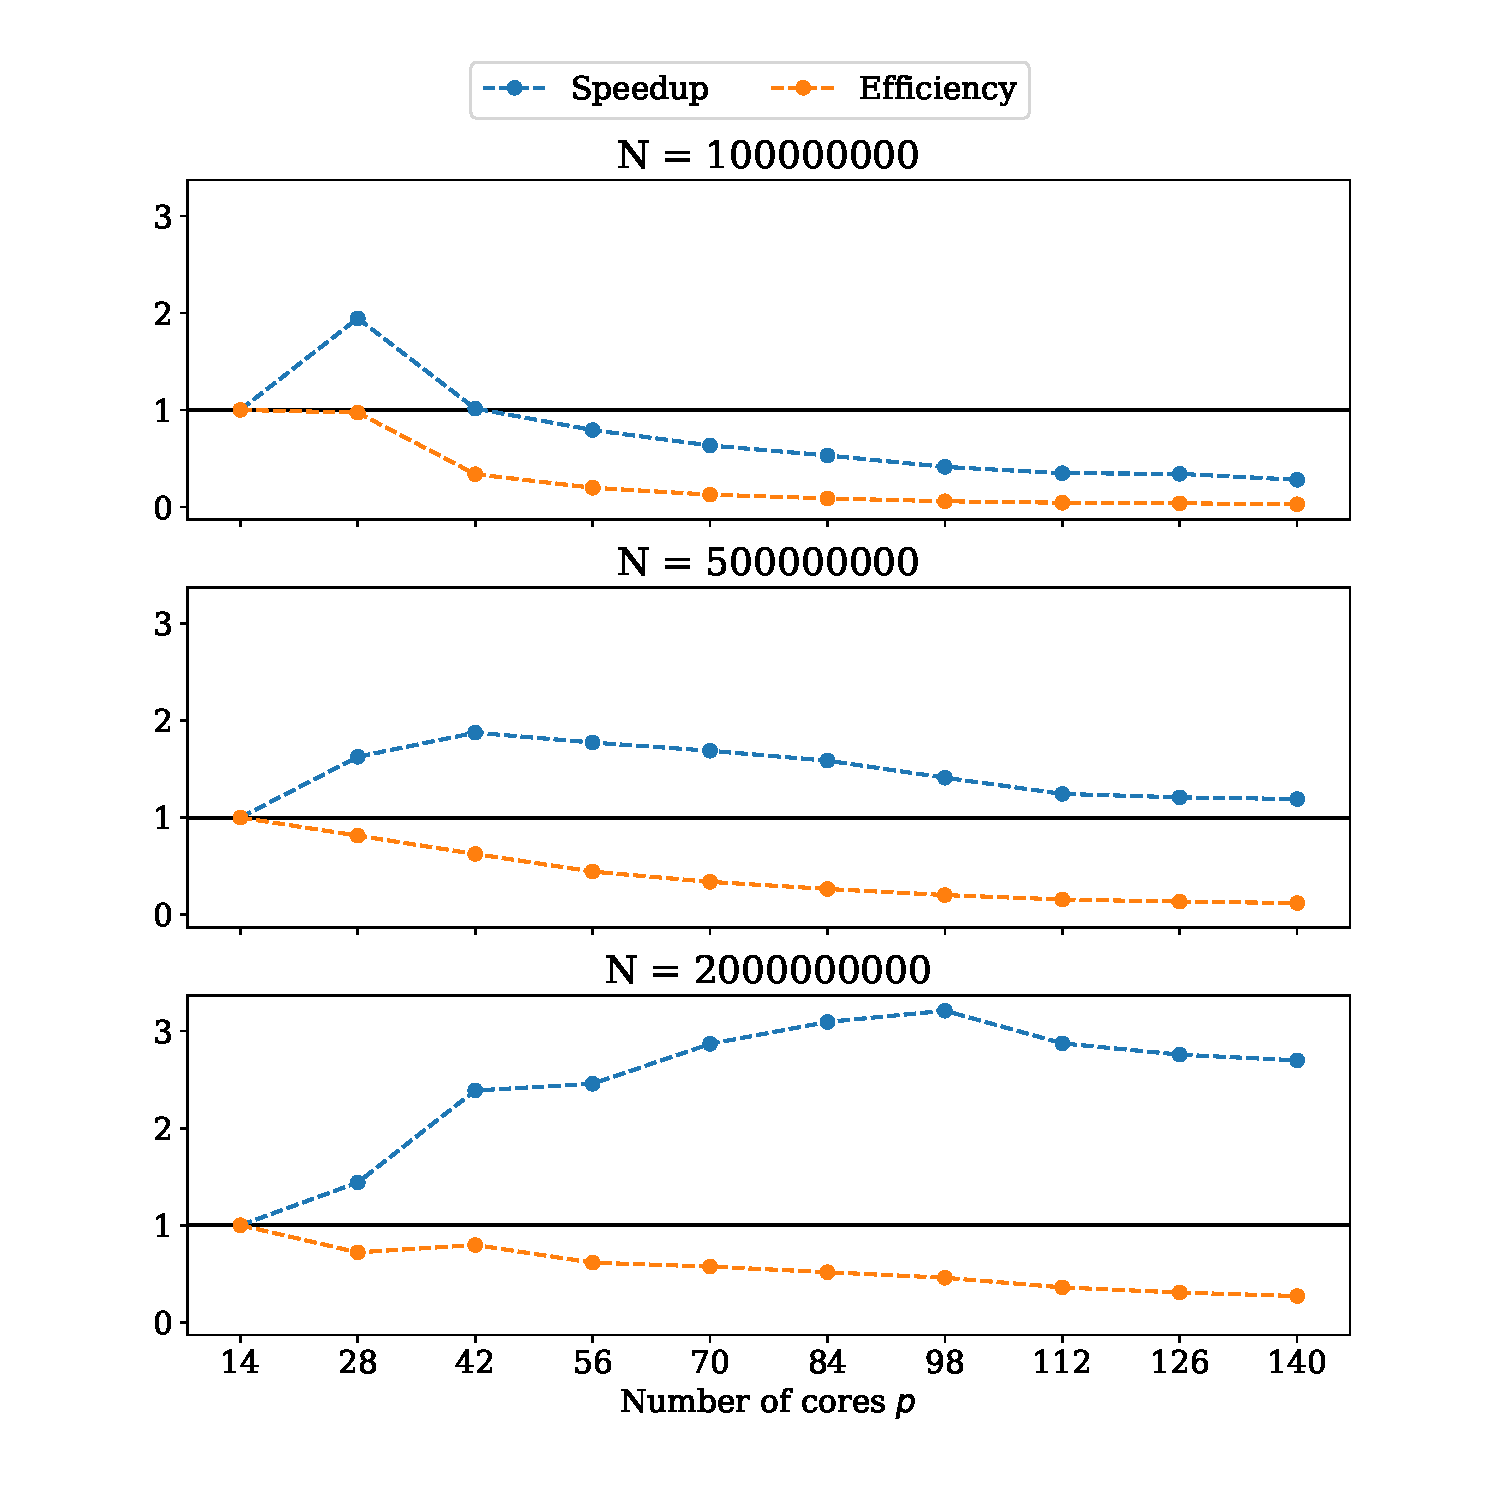
\includegraphics[width=\textwidth]{../part_1/plot/v2_speedup.pdf}
  \caption{Speedup and efficiency of \textit{bucket\_sort\_v2.c} for different
    number of cores $p$.}
  \label{fig:p1_v2_speedup}
\end{figure}
\begin{figure}
  \centering
  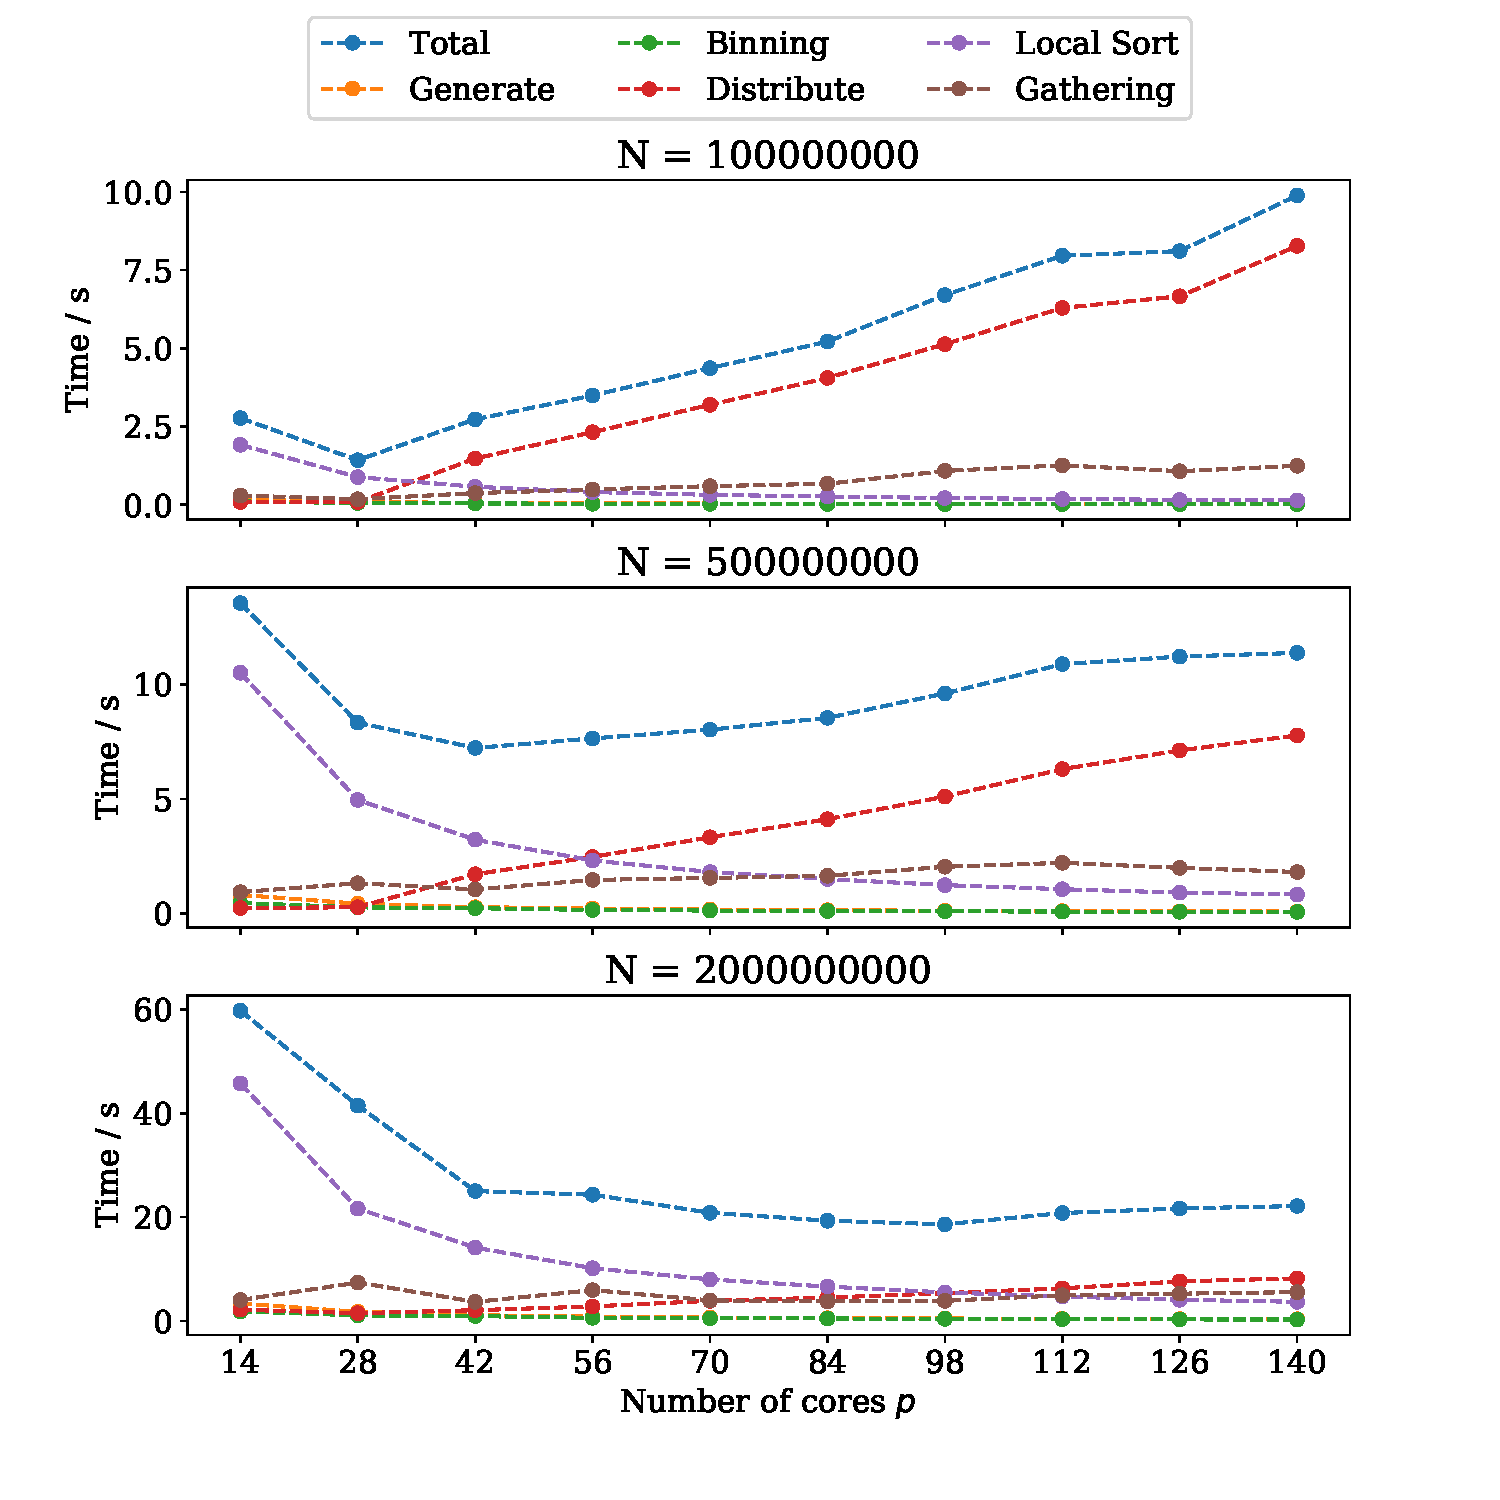
\includegraphics[width=\textwidth]{../part_1/plot/v2_times.pdf}
  \caption{Execution times of \textit{bucket\_sort\_v2.c} for different number
  of cores $p$.}
  \label{fig:p1_v2_times}
\end{figure}
\FloatBarrier

\section*{Part 2}
\subsection*{1.}
I find plots generally a lot more helpful than tables, so I went with that.
Figure~\ref{fig:p2_v2_load_balance} and
Figure~\ref{fig:p2_v2_square_load_balance} show the load balance in terms of
spread in execution time for the uniform and squared versions respectively.
Comparing the two clearly proofs we have a load imbalance problem: The spread
between the minimal, average and maximal execution times is significantly
larger for the squared distribution. This is of course the case because smaller
numbers are quadratically more likely there, resulting in quadratically less
work for higher ranked processes. The speedup and efficiency curves for the
squared distribution can be seen in Figure~\ref{fig:p2_v2_square_speedup} and
the partial execution times are shown in Figure~\ref{fig:p2_v2_square_times}.

\begin{figure}
  \centering
  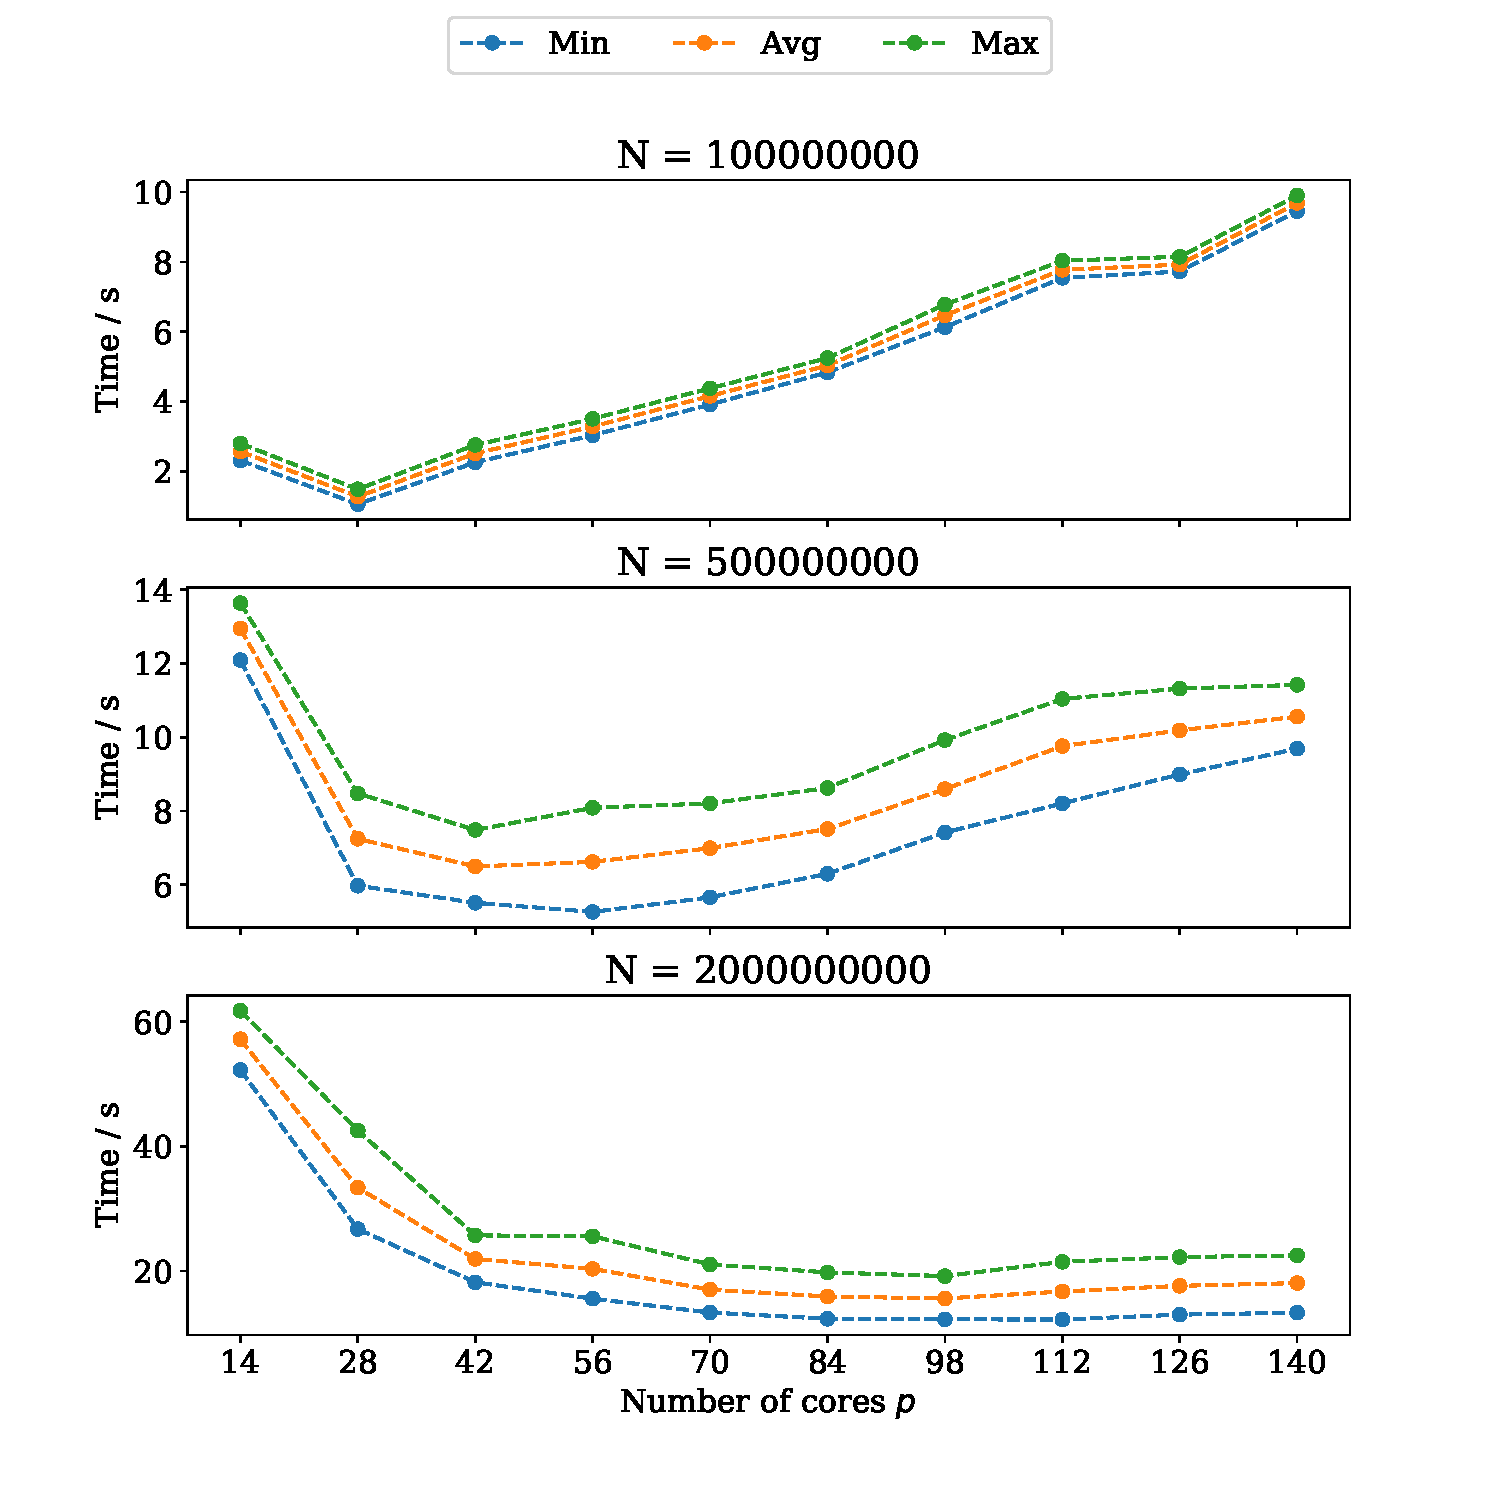
\includegraphics[width=\textwidth]{../part_2/plot/v2_load_balance.pdf}
  \caption{Load balance of \textit{bucket\_sort\_v2.c} for different number of
  cores $p$.}
  \label{fig:p2_v2_load_balance}
\end{figure}
\begin{figure}
  \centering
  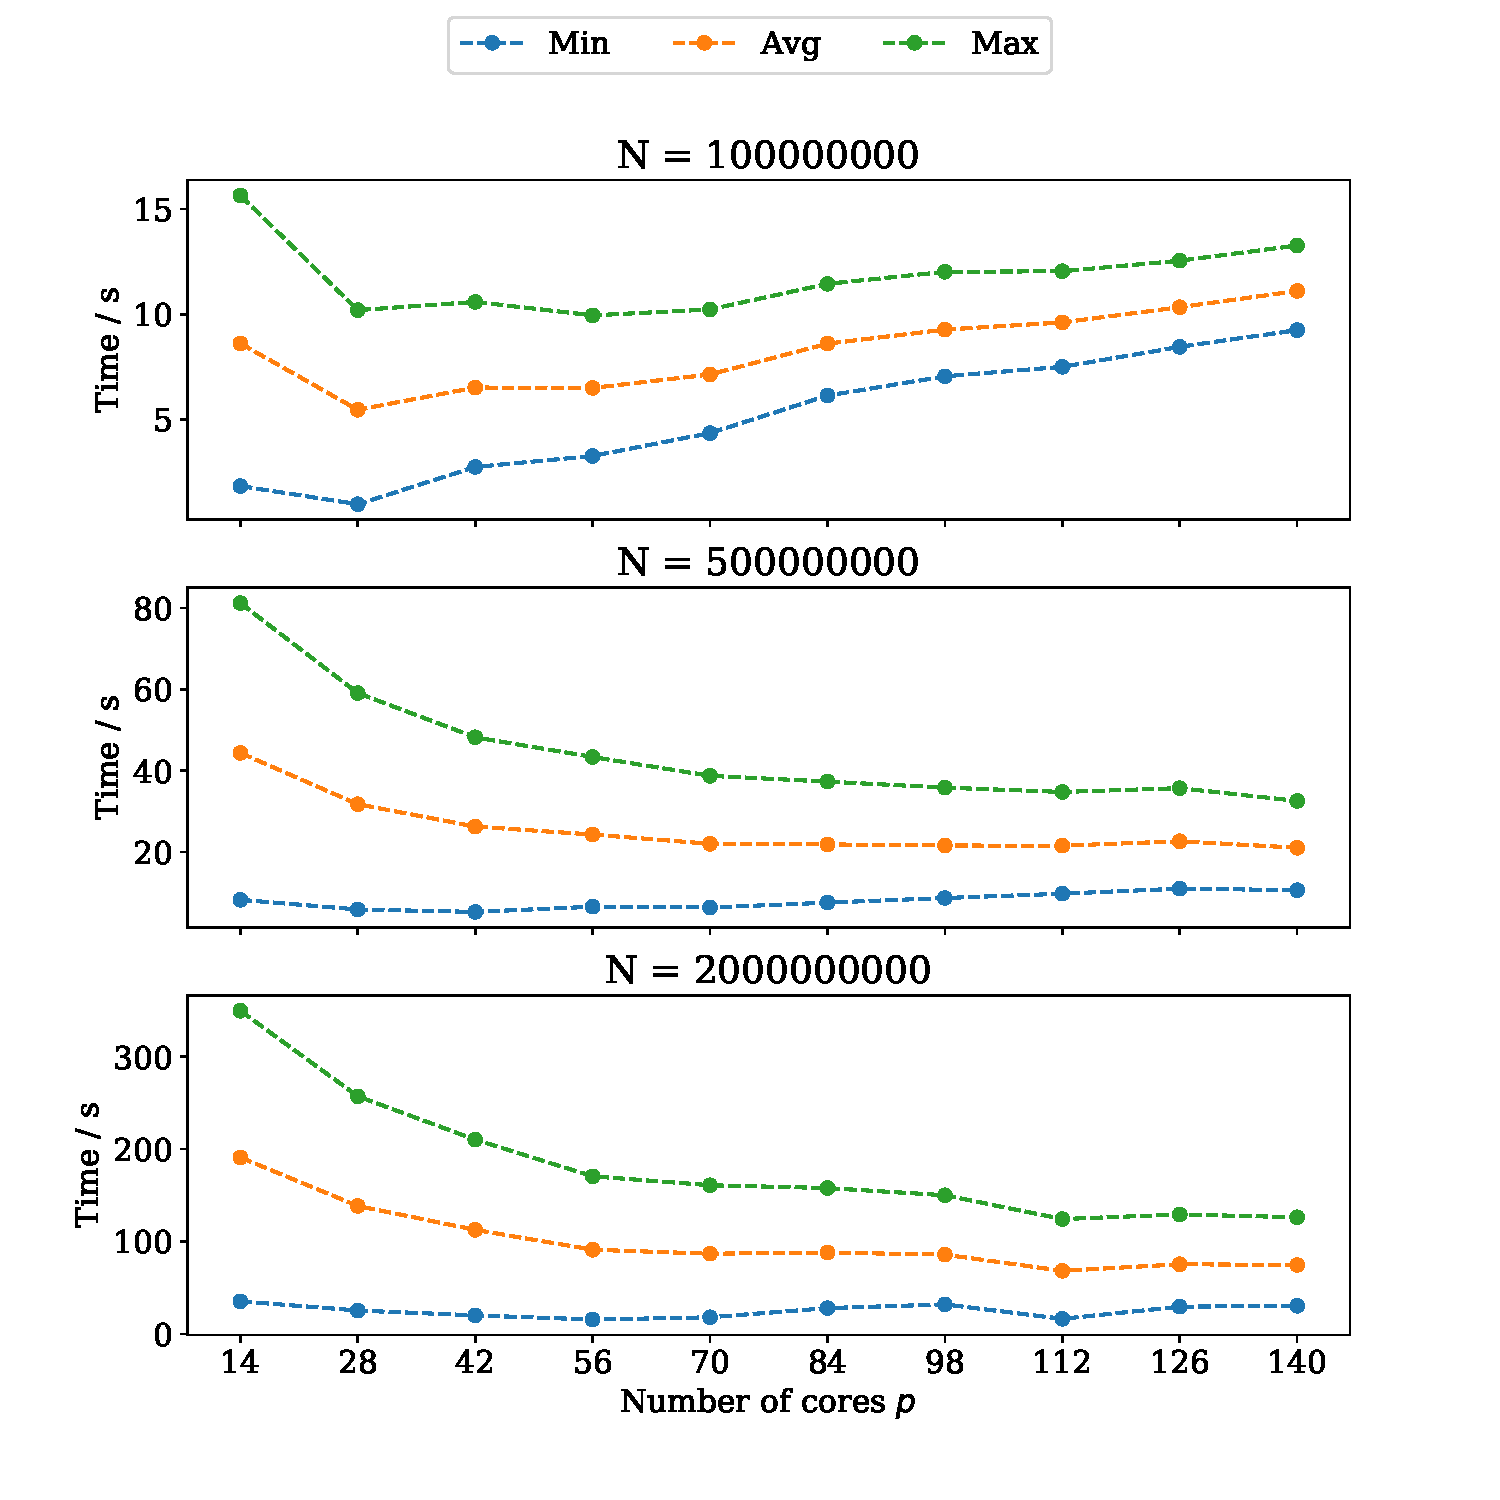
\includegraphics[width=\textwidth]{../part_2/plot/v2_square_load_balance.pdf}
  \caption{Load balance of \textit{bucket\_sort\_v2\_square.c} for different
  number of cores $p$.}
  \label{fig:p2_v2_square_load_balance}
\end{figure}
\begin{figure}
  \centering
  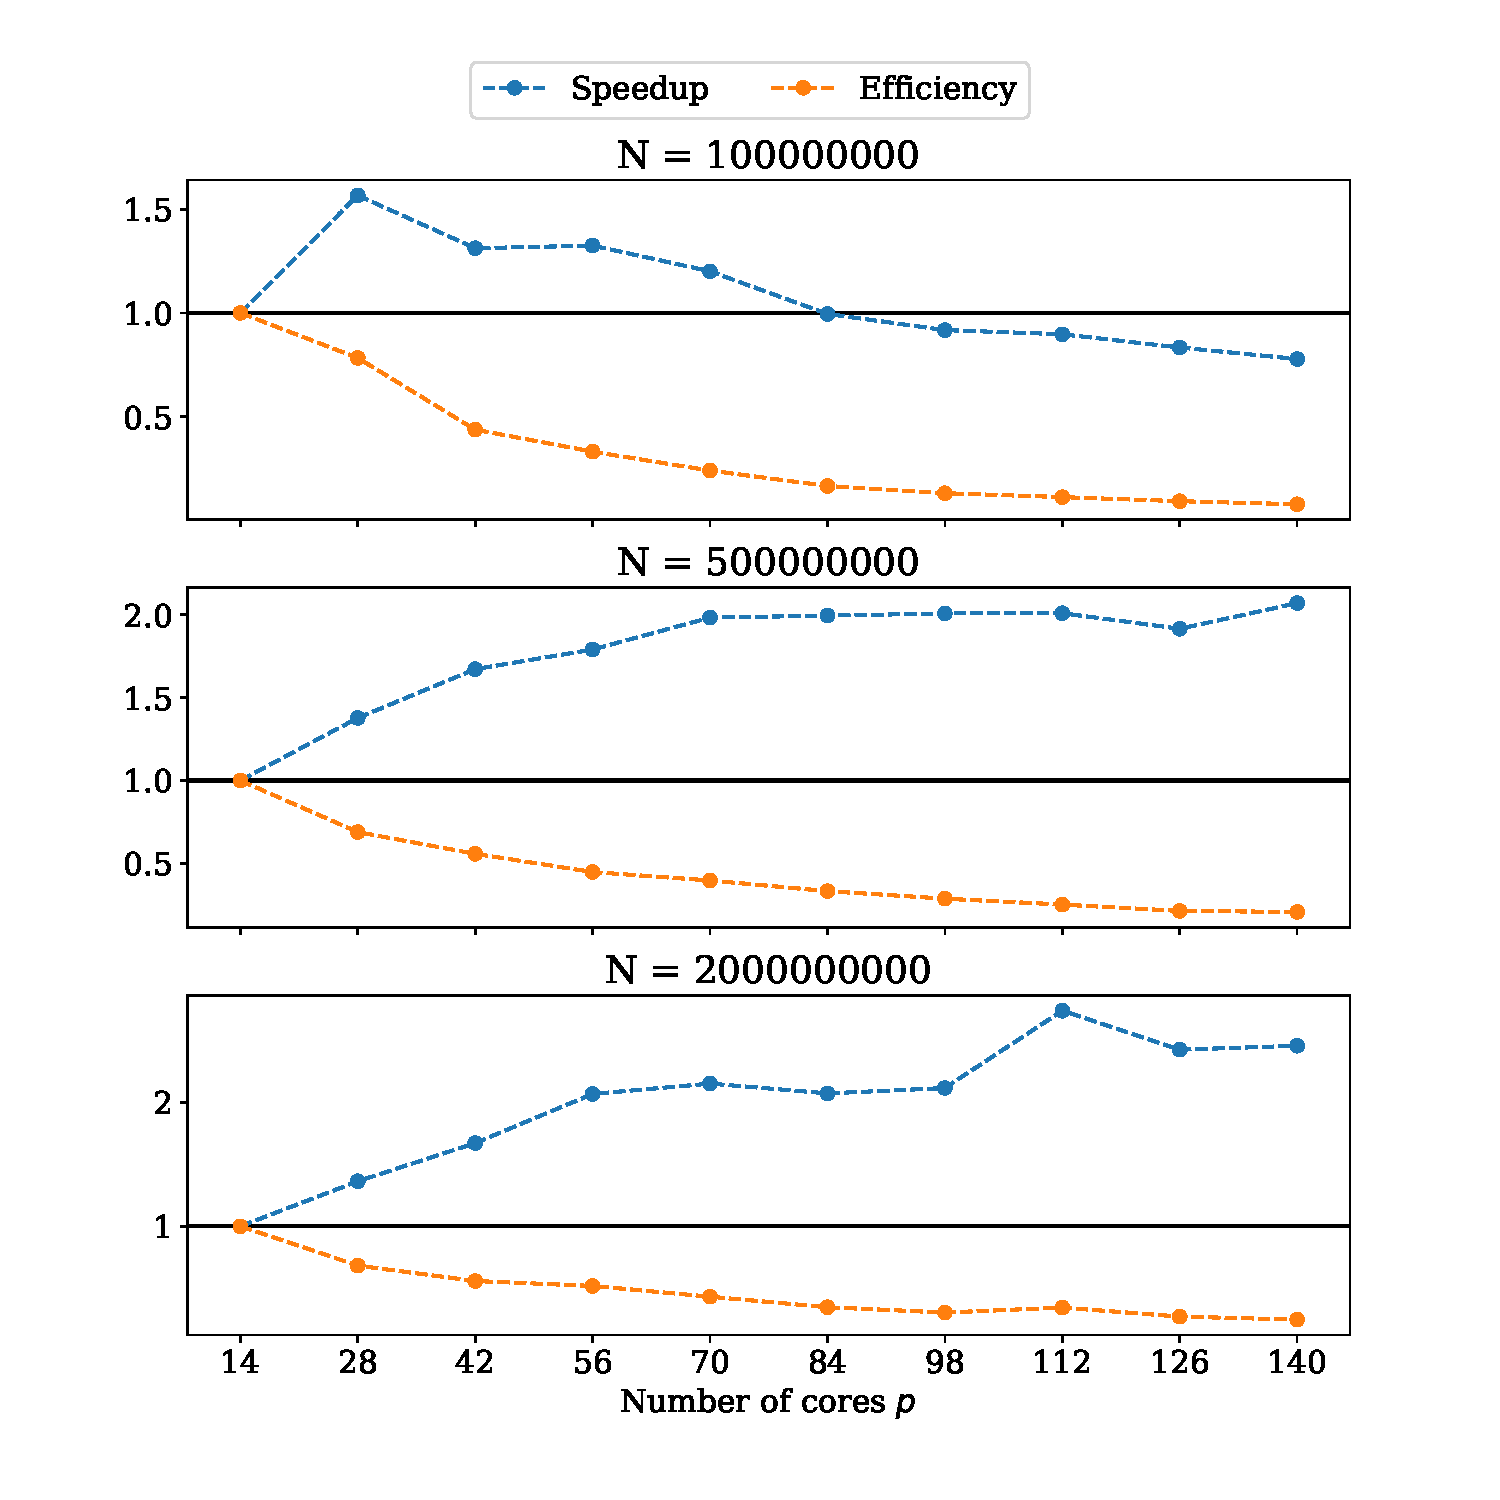
\includegraphics[width=\textwidth]{../part_2/plot/v2_square_speedup.pdf}
  \caption{Speedup and efficiency of \textit{bucket\_sort\_v2\_square.c} for
  different number of cores $p$.}
  \label{fig:p2_v2_square_speedup}
\end{figure}
\begin{figure}
  \centering
  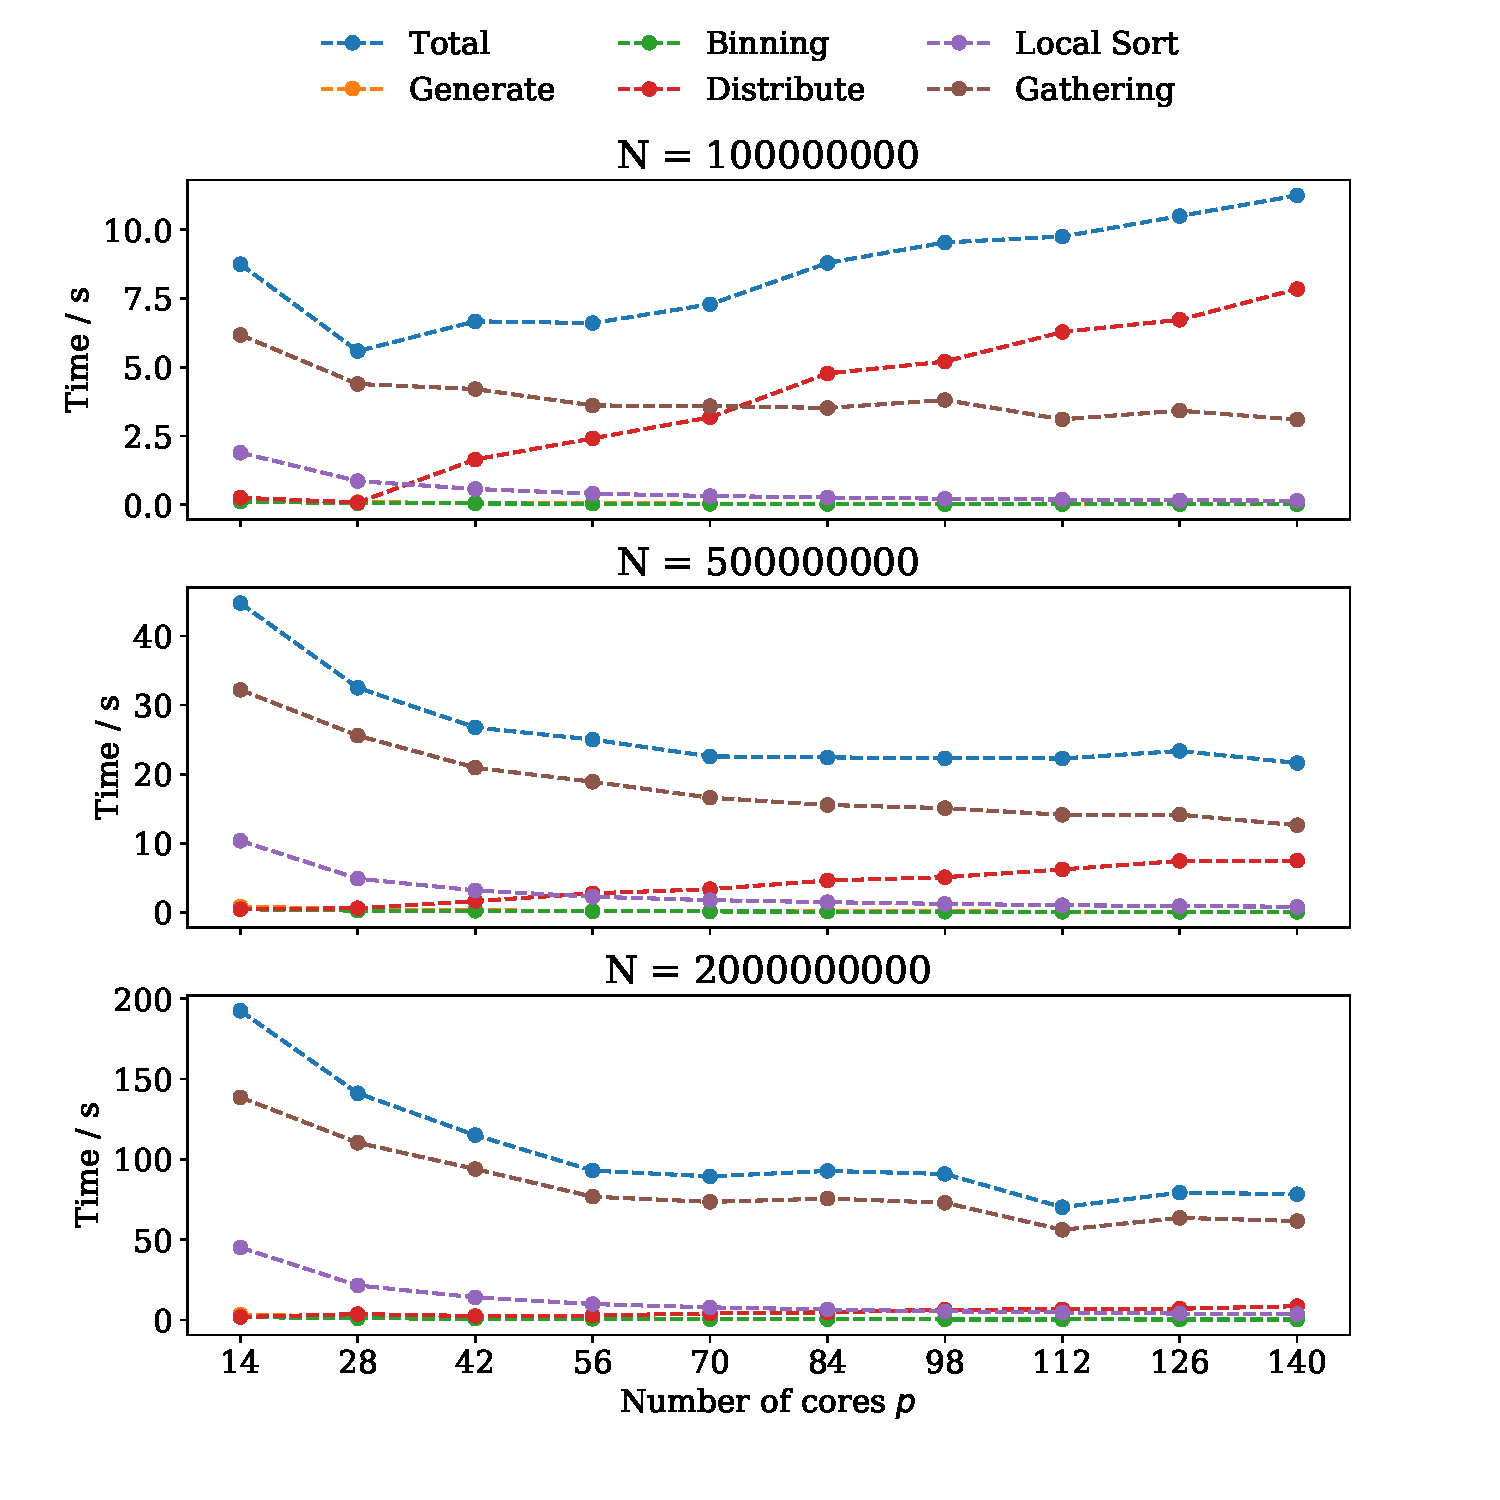
\includegraphics[width=\textwidth]{../part_2/plot/v2_square_times.pdf}
  \caption{Execution times of \textit{bucket\_sort\_v2\_square.c} for different
  number of cores $p$.}
  \label{fig:p2_v2_square_times}
\end{figure}
\FloatBarrier

\subsection*{2.}
See code in repository. For some reason there is no 3. so let's continue with
4.\,.

\subsection*{4.}
I assume here you mean speedup over the v2 squared distribution case, which is
provided by Figure~\ref{fig:p2_v3_speedup}. We can clearly see a large speedup,
which indicates we remedied the load imbalance problem. I also provide a
speedup and efficiency curve with using one socket with v3 as base case in
Figure~\ref{fig:p2_v3_speedup_v3_base}, which is not really helpful here
though. It is pretty much the same as for v2 which just tells us it scales the
same way, which makes sense.

\begin{figure}
  \centering
  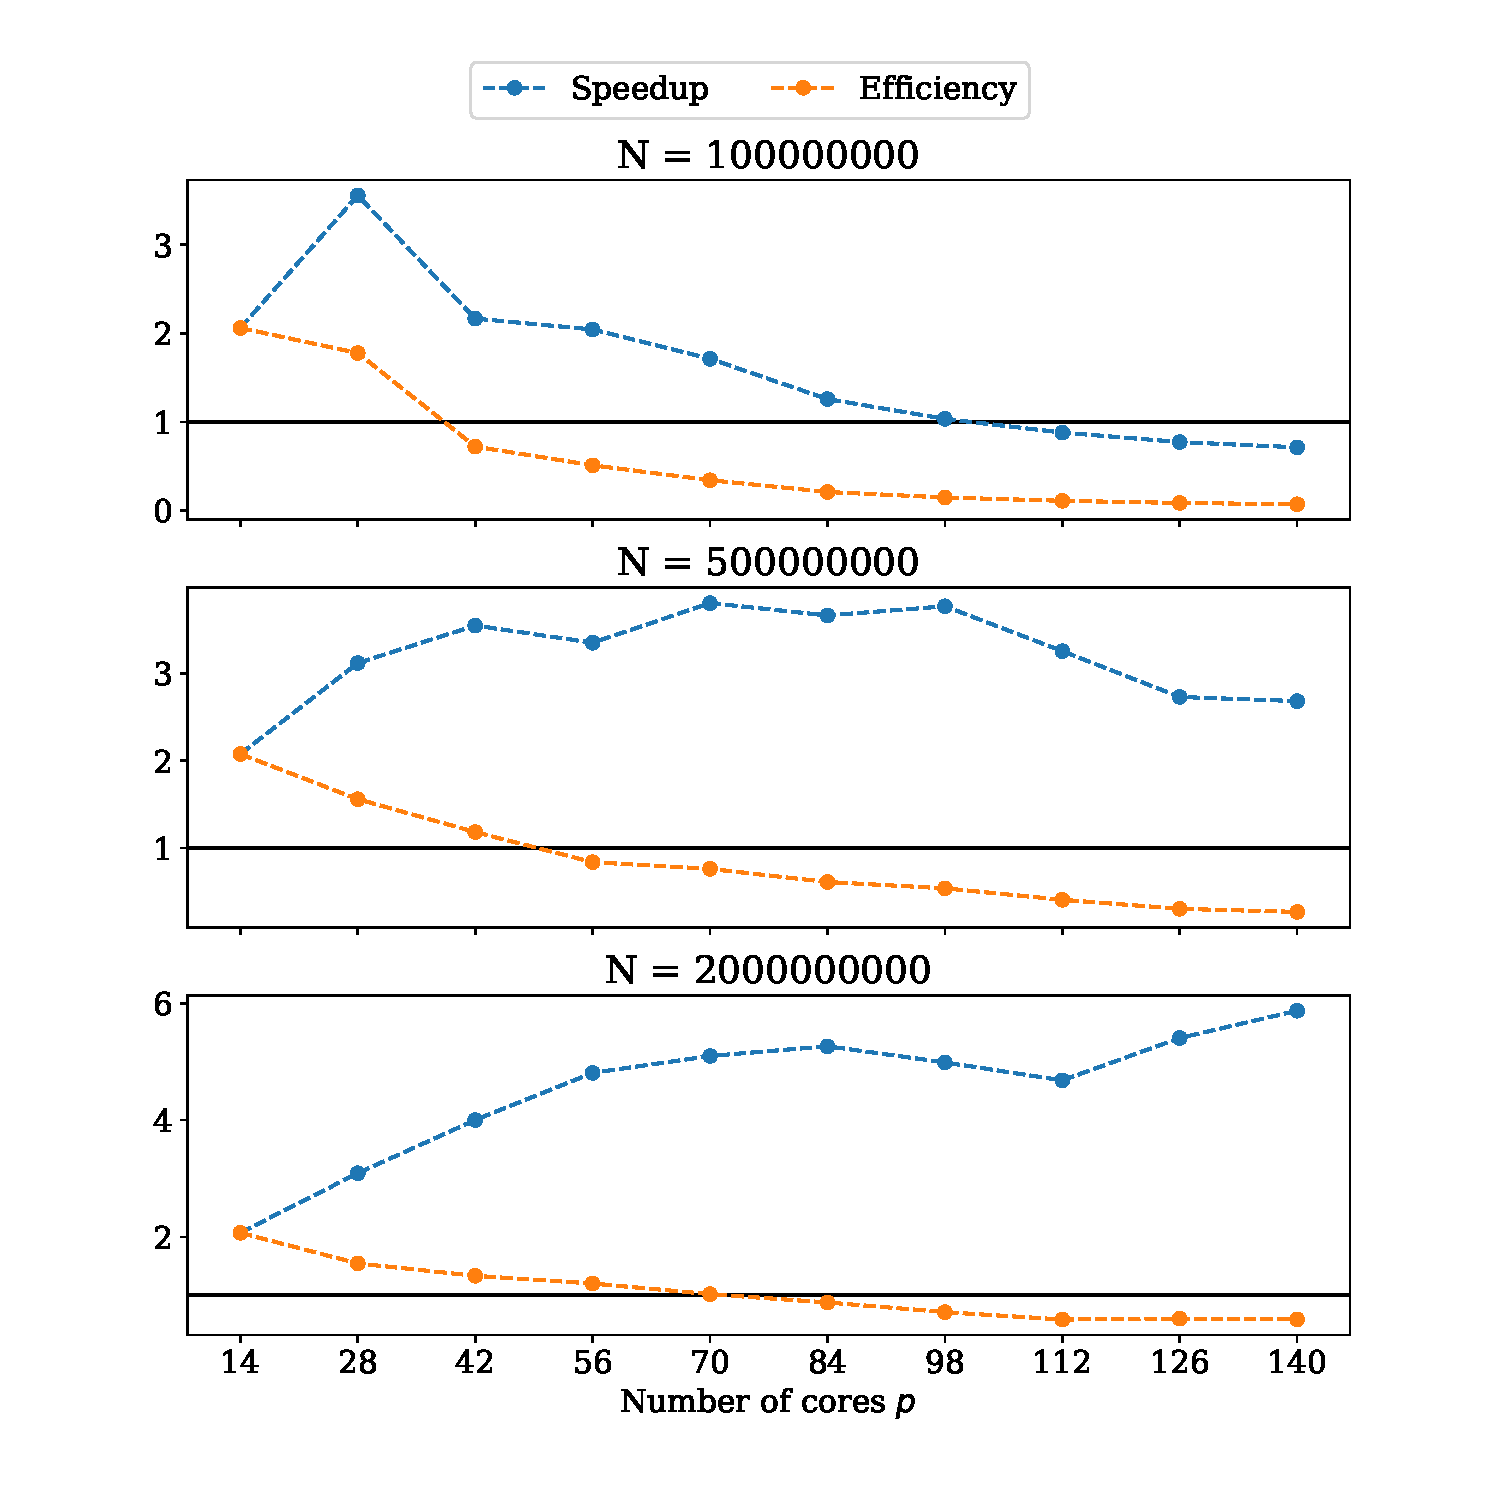
\includegraphics[width=\textwidth]{../part_2/plot/v3_speedup.pdf}
  \caption{Speedup and efficiency of \textit{bucket\_sort\_v3.c} for different
  number of cores $p$ with $p=14$ of \textit{bucket\_sort\_v2\_square.c} being
  the base case.}
  \label{fig:p2_v3_speedup}
\end{figure}
\begin{figure}
  \centering
  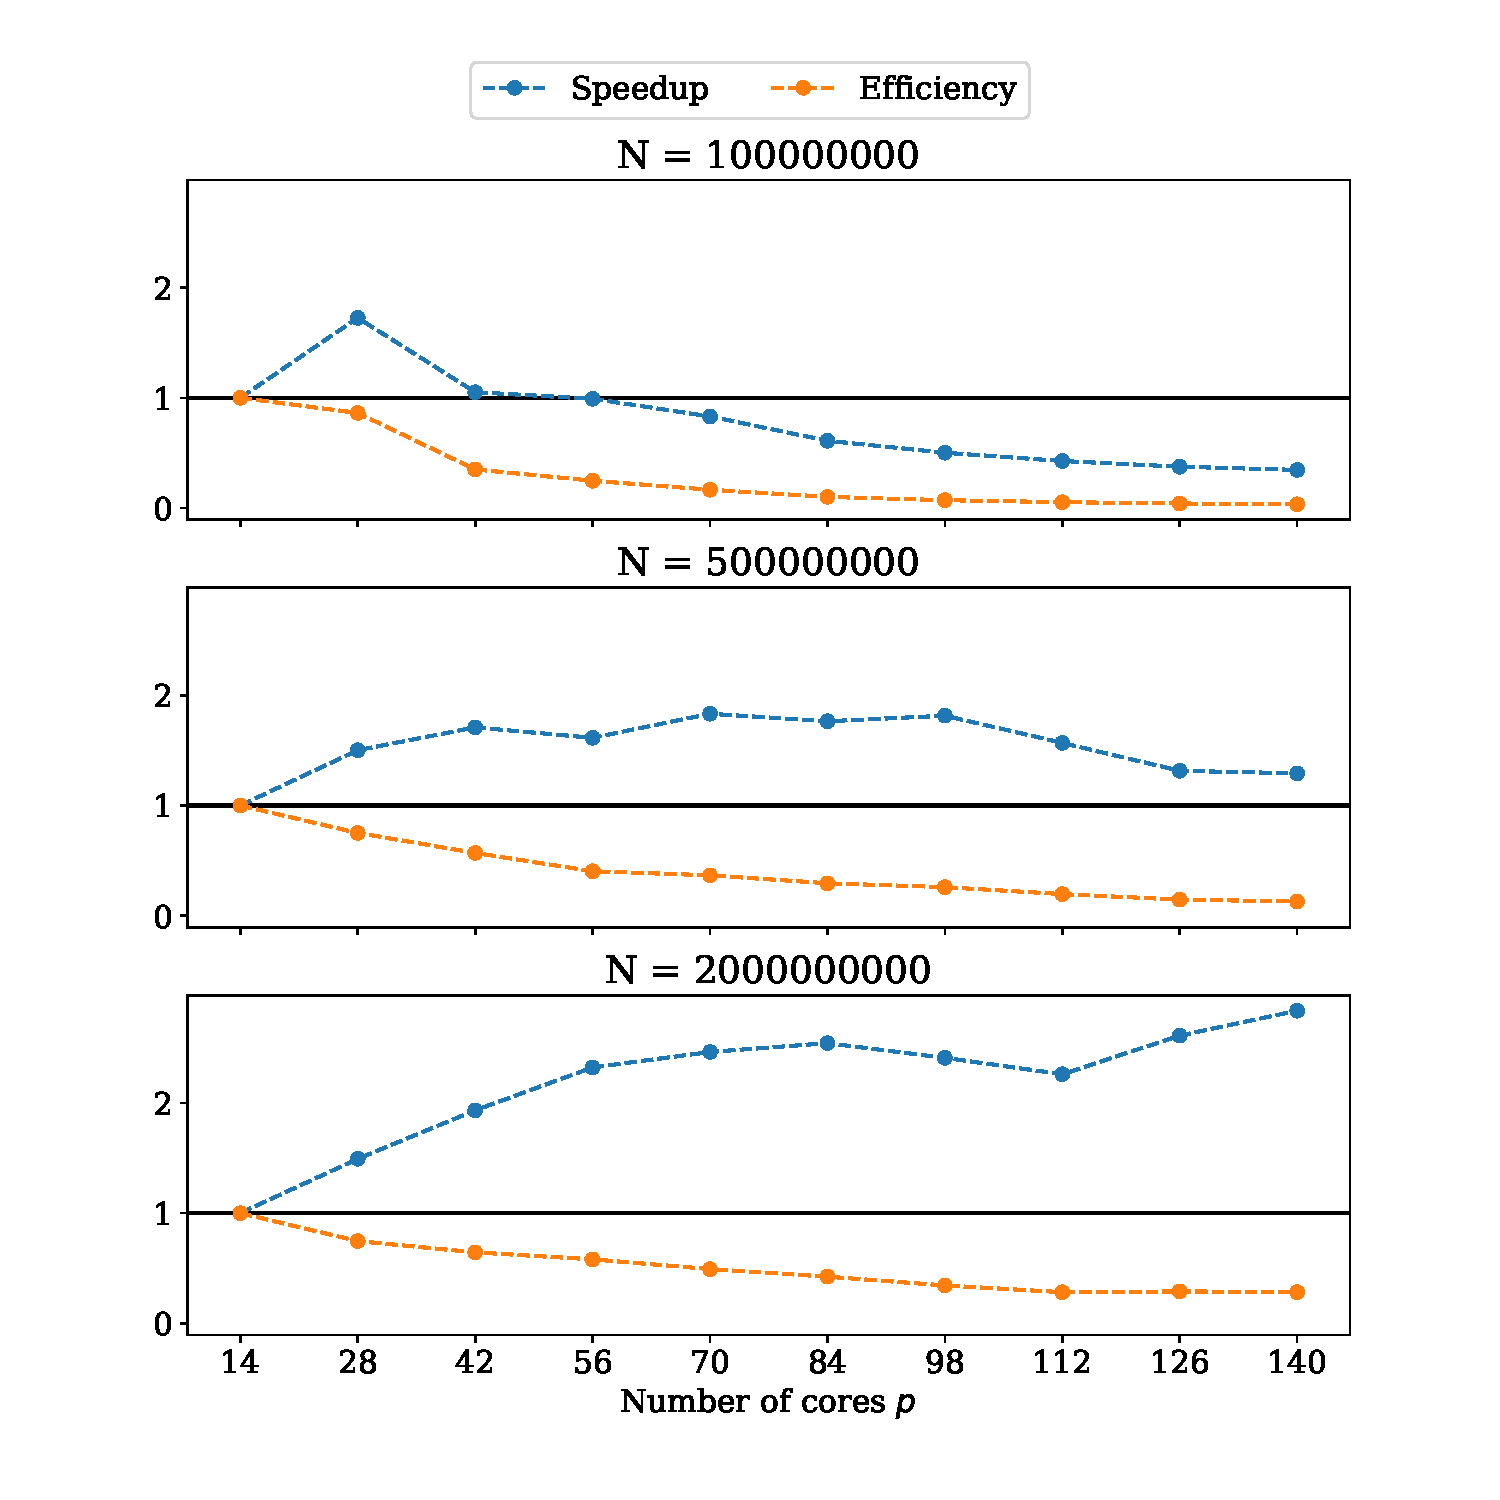
\includegraphics[width=\textwidth]{../part_2/plot/v3_speedup_v3_base.pdf}
  \caption{Speedup and efficiency of \textit{bucket\_sort\_v3.c} for different
  number of cores $p$.}
  \label{fig:p2_v3_speedup_v3_base}
\end{figure}

\subsection*{5.}
The time spend in different parts of the program is shown in
Figure~\ref{fig:p2_v3_times}. In all cases, selecting the pivots does not take
any significant amount of time (about one second). This includes the
communication time.

Taking all this into account: Yes, generally the time spent in selecting pivots
is absolutely worth it. Once again, only for small problem sizes the overhead
can become a problem (see Figure~\ref{fig:p2_v3_speedup}).

Additional comment: Obviously here it does make a lot more sense to just
statically rescale the bin sizes instead of dynamically choosing pivots.
However, I get the point you want to teach here, this only works in case one
knows the actual distribution. For highly variable input data with unknown
distribution the pivoting method will generally be of advantage.

\begin{figure}
  \centering
  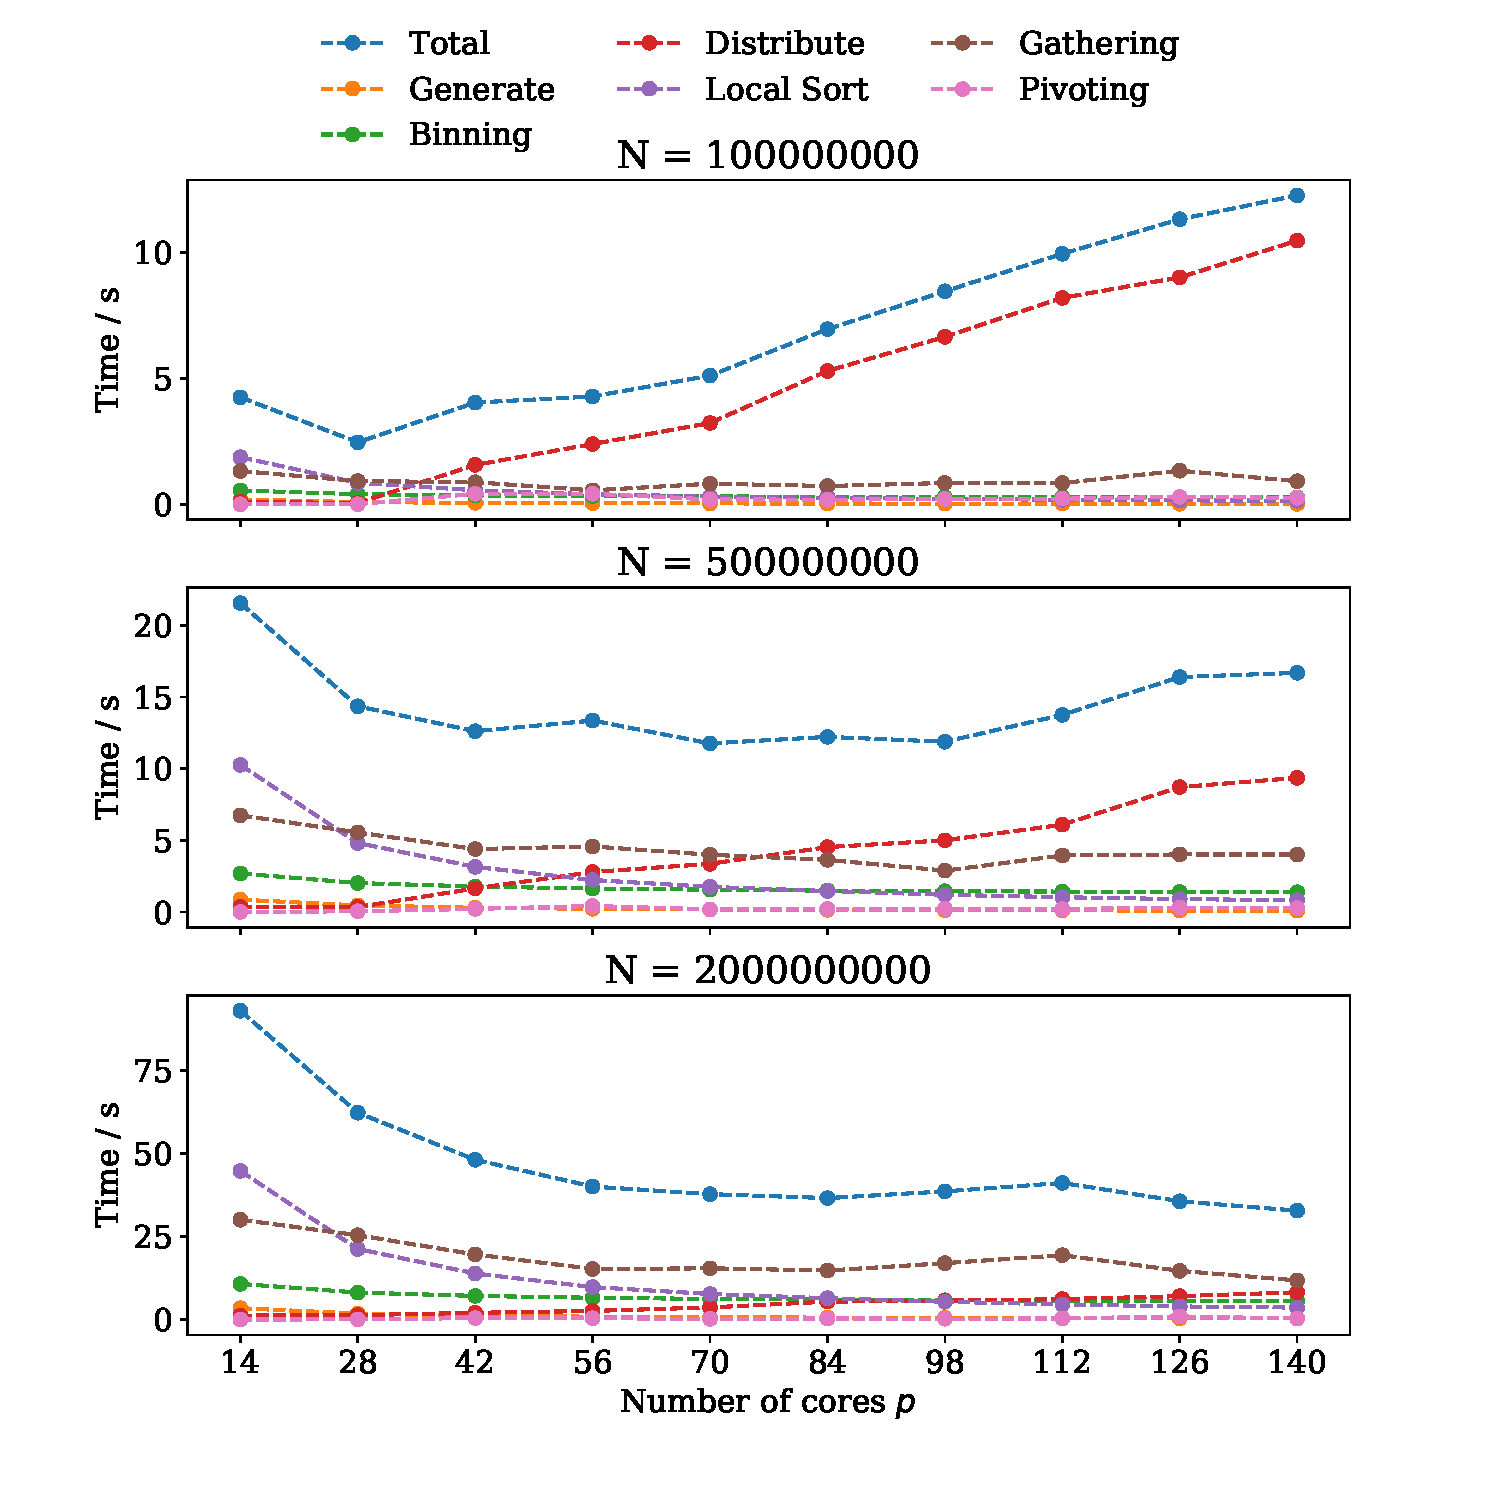
\includegraphics[width=\textwidth]{../part_2/plot/v3_times.pdf}
  \caption{Execution times  of \textit{bucket\_sort\_v3.c} for different number
  of cores $p$.}
  \label{fig:p2_v3_times}
\end{figure}
\end{document}
